% Options for packages loaded elsewhere
\PassOptionsToPackage{unicode}{hyperref}
\PassOptionsToPackage{hyphens}{url}
%
\documentclass[
]{book}
\usepackage{lmodern}
\usepackage{amssymb,amsmath}
\usepackage{ifxetex,ifluatex}
\ifnum 0\ifxetex 1\fi\ifluatex 1\fi=0 % if pdftex
  \usepackage[T1]{fontenc}
  \usepackage[utf8]{inputenc}
  \usepackage{textcomp} % provide euro and other symbols
\else % if luatex or xetex
  \usepackage{unicode-math}
  \defaultfontfeatures{Scale=MatchLowercase}
  \defaultfontfeatures[\rmfamily]{Ligatures=TeX,Scale=1}
\fi
% Use upquote if available, for straight quotes in verbatim environments
\IfFileExists{upquote.sty}{\usepackage{upquote}}{}
\IfFileExists{microtype.sty}{% use microtype if available
  \usepackage[]{microtype}
  \UseMicrotypeSet[protrusion]{basicmath} % disable protrusion for tt fonts
}{}
\makeatletter
\@ifundefined{KOMAClassName}{% if non-KOMA class
  \IfFileExists{parskip.sty}{%
    \usepackage{parskip}
  }{% else
    \setlength{\parindent}{0pt}
    \setlength{\parskip}{6pt plus 2pt minus 1pt}}
}{% if KOMA class
  \KOMAoptions{parskip=half}}
\makeatother
\usepackage{xcolor}
\IfFileExists{xurl.sty}{\usepackage{xurl}}{} % add URL line breaks if available
\IfFileExists{bookmark.sty}{\usepackage{bookmark}}{\usepackage{hyperref}}
\hypersetup{
  pdftitle={RStudio 2020 Internship Application},
  pdfauthor={Riccardo Esclapon},
  hidelinks,
  pdfcreator={LaTeX via pandoc}}
\urlstyle{same} % disable monospaced font for URLs
\usepackage{color}
\usepackage{fancyvrb}
\newcommand{\VerbBar}{|}
\newcommand{\VERB}{\Verb[commandchars=\\\{\}]}
\DefineVerbatimEnvironment{Highlighting}{Verbatim}{commandchars=\\\{\}}
% Add ',fontsize=\small' for more characters per line
\usepackage{framed}
\definecolor{shadecolor}{RGB}{248,248,248}
\newenvironment{Shaded}{\begin{snugshade}}{\end{snugshade}}
\newcommand{\AlertTok}[1]{\textcolor[rgb]{0.94,0.16,0.16}{#1}}
\newcommand{\AnnotationTok}[1]{\textcolor[rgb]{0.56,0.35,0.01}{\textbf{\textit{#1}}}}
\newcommand{\AttributeTok}[1]{\textcolor[rgb]{0.77,0.63,0.00}{#1}}
\newcommand{\BaseNTok}[1]{\textcolor[rgb]{0.00,0.00,0.81}{#1}}
\newcommand{\BuiltInTok}[1]{#1}
\newcommand{\CharTok}[1]{\textcolor[rgb]{0.31,0.60,0.02}{#1}}
\newcommand{\CommentTok}[1]{\textcolor[rgb]{0.56,0.35,0.01}{\textit{#1}}}
\newcommand{\CommentVarTok}[1]{\textcolor[rgb]{0.56,0.35,0.01}{\textbf{\textit{#1}}}}
\newcommand{\ConstantTok}[1]{\textcolor[rgb]{0.00,0.00,0.00}{#1}}
\newcommand{\ControlFlowTok}[1]{\textcolor[rgb]{0.13,0.29,0.53}{\textbf{#1}}}
\newcommand{\DataTypeTok}[1]{\textcolor[rgb]{0.13,0.29,0.53}{#1}}
\newcommand{\DecValTok}[1]{\textcolor[rgb]{0.00,0.00,0.81}{#1}}
\newcommand{\DocumentationTok}[1]{\textcolor[rgb]{0.56,0.35,0.01}{\textbf{\textit{#1}}}}
\newcommand{\ErrorTok}[1]{\textcolor[rgb]{0.64,0.00,0.00}{\textbf{#1}}}
\newcommand{\ExtensionTok}[1]{#1}
\newcommand{\FloatTok}[1]{\textcolor[rgb]{0.00,0.00,0.81}{#1}}
\newcommand{\FunctionTok}[1]{\textcolor[rgb]{0.00,0.00,0.00}{#1}}
\newcommand{\ImportTok}[1]{#1}
\newcommand{\InformationTok}[1]{\textcolor[rgb]{0.56,0.35,0.01}{\textbf{\textit{#1}}}}
\newcommand{\KeywordTok}[1]{\textcolor[rgb]{0.13,0.29,0.53}{\textbf{#1}}}
\newcommand{\NormalTok}[1]{#1}
\newcommand{\OperatorTok}[1]{\textcolor[rgb]{0.81,0.36,0.00}{\textbf{#1}}}
\newcommand{\OtherTok}[1]{\textcolor[rgb]{0.56,0.35,0.01}{#1}}
\newcommand{\PreprocessorTok}[1]{\textcolor[rgb]{0.56,0.35,0.01}{\textit{#1}}}
\newcommand{\RegionMarkerTok}[1]{#1}
\newcommand{\SpecialCharTok}[1]{\textcolor[rgb]{0.00,0.00,0.00}{#1}}
\newcommand{\SpecialStringTok}[1]{\textcolor[rgb]{0.31,0.60,0.02}{#1}}
\newcommand{\StringTok}[1]{\textcolor[rgb]{0.31,0.60,0.02}{#1}}
\newcommand{\VariableTok}[1]{\textcolor[rgb]{0.00,0.00,0.00}{#1}}
\newcommand{\VerbatimStringTok}[1]{\textcolor[rgb]{0.31,0.60,0.02}{#1}}
\newcommand{\WarningTok}[1]{\textcolor[rgb]{0.56,0.35,0.01}{\textbf{\textit{#1}}}}
\usepackage{longtable,booktabs}
% Correct order of tables after \paragraph or \subparagraph
\usepackage{etoolbox}
\makeatletter
\patchcmd\longtable{\par}{\if@noskipsec\mbox{}\fi\par}{}{}
\makeatother
% Allow footnotes in longtable head/foot
\IfFileExists{footnotehyper.sty}{\usepackage{footnotehyper}}{\usepackage{footnote}}
\makesavenoteenv{longtable}
\usepackage{graphicx,grffile}
\makeatletter
\def\maxwidth{\ifdim\Gin@nat@width>\linewidth\linewidth\else\Gin@nat@width\fi}
\def\maxheight{\ifdim\Gin@nat@height>\textheight\textheight\else\Gin@nat@height\fi}
\makeatother
% Scale images if necessary, so that they will not overflow the page
% margins by default, and it is still possible to overwrite the defaults
% using explicit options in \includegraphics[width, height, ...]{}
\setkeys{Gin}{width=\maxwidth,height=\maxheight,keepaspectratio}
% Set default figure placement to htbp
\makeatletter
\def\fps@figure{htbp}
\makeatother
\setlength{\emergencystretch}{3em} % prevent overfull lines
\providecommand{\tightlist}{%
  \setlength{\itemsep}{0pt}\setlength{\parskip}{0pt}}
\setcounter{secnumdepth}{5}
\usepackage{booktabs}
\usepackage[]{natbib}
\bibliographystyle{apalike}

\title{RStudio 2020 Internship Application}
\author{Riccardo Esclapon}
\date{}

\begin{document}
\maketitle

{
\setcounter{tocdepth}{1}
\tableofcontents
}
\hypertarget{overview}{%
\chapter{Overview}\label{overview}}

Video intro here

\url{https://education.rstudio.com/blog/2020/02/applications-for-2020-intern-program-are-now-open/}

APPLICATIONS END ON MARCH 5TH BE SURE TO APPLY BEFORE THEN!!

For video:

Start off with overview of projects I am suited for showing work I did for this application specifically. Then go on to talk about ways I have applied the broad RMarkdown ecosystem and automation in my work. Then talk a bit more about myself. Talk about ideal tutorial overview and close things by mentioning cool charts/visualizations section (outline this at a high level under 2 minutes in the video at the start here)

\hypertarget{fit}{%
\chapter{What makes me a good fit}\label{fit}}

Here are some of the things I believe make me a great fit for the internship:

\hypertarget{i-uxfe0f-.rmd-files}{%
\section{I ❤️ .Rmd files}\label{i-uxfe0f-.rmd-files}}

I was completely blown away by the R Markdown file format when I first discovered it, and I definitely felt a bit cheated by the fact that none of the courses I took during my undergrad in R mentioned it at all or the tidyverse. I have spent a lot of my time learning R Markdown and digging through books and amazing resources made available by RStudio, so here are some of my favorite formats that I would love to make more content around and teach people about:

\hypertarget{learnr}{%
\subsection{Learnr}\label{learnr}}

I first discovered the \textbf{\emph{learnr}} \citep{R-learnr} package in late 2018 and was really impressed by the functionality it provides. My first real project using learnr was centered around teaching my young Italian cousins to program in R by allowing them to compare their Fortnite stats in real time to each other and the best players in the world, and be able to learn more about the game through working with data, for example finding the best weapon based on their damage and range. The GitHub repository associated with that project can be found here: \url{https://github.com/ries9112/R-Tutorial} (the apps themselves are down but the repo has some gifs illustrating the past functionality)

\textbf{More recently, I have been using learnr to offer tutorials on my website using learnr where every time the tutorial is opened, users learn to program in R using data from the cryptocurrency markets that is never outdated by more than 1 hour:}

(this takes about 45 seconds to load, give it more time if it's showing up blank)

\hypertarget{bookdown}{%
\subsection{Bookdown}\label{bookdown}}

At one point I was very close to paying for a monthly subscription on gitbook.com because I thought it was such an amazing format to provide documentation through, so I was particularly impressed by and grateful for the bookdown \citep{R-bookdown} package, and these days it's my go to for organizing most things I work on, so why not my application?

This document is obviously an example of a bookdown document in itself, but here's another guide I put together using bookdown:

\emph{MAKE SURE THIS ACTUALLY REFRESHES WITH GITHUB ACTIONS BEFORE APPLYING}

I also found that documentation done in bookdown can work really great when working within a large company as well, and I put together some very thorough documentation for a project using bookdown that was very well received (but I can't show here). In my particular case it worked really well because I could send the link to the html index of the bookdown document and when opened it would behave like a website hosted on the shared folders within the secure network which ended up being particularly simple and effective.

\hypertarget{presentations}{%
\subsection{Presentations}\label{presentations}}

I am a \textbf{big} fan of ioslides and revealjs in particular as R Markdown outputs. I find the revealjs output to be incredibly cool with the rotating cube animation, and the ability to not only move forward but move downward adds a surprisingly useful tool to break down topics; ioslides is just really clean, well made and easy to use and looks great with widescreen enabled. I aspire to be an expert in Xaringan one day but am not currently.

Making presentations in R Markdown is what really got me working with .Rmd files, because I started working towards a very specific project using an idea I haven't really seen elsewhere of creating presentations that give the user options and as they make their way through the slides, those options affect not only what they see in the slides that come afterwards, but also the options they are given. For example, the user could choose to do an analysis for a particular asset, then choose the main category of the analysis to perform, then the sub-category of the analysis and so on, until by the end of the presentation the user has performed an analysis that was completely unique and tailored to their preferences and interests. See the gif below for an example of what this looks like:

\hypertarget{blogdown}{%
\subsection{Blogdown}\label{blogdown}}

Blogdown\citep{R-blogdown} and bookdown work very similarly, so most of what I mentioned in the \protect\hyperlink{bookdown}{bookdown section} applies here. Because my website predictcrypto.com only shows the latest data based on the current date, I leverage blogdown to create weekly snapshots of the visualizations over the last 7 day period: \url{https://predictcryptoblog.com/}.

Because all these systems work so well with automation, as I keep adding new interesting content to my website I can also add archives of that content using blogdown.

\hypertarget{pagedown}{%
\subsection{Pagedown}\label{pagedown}}

Pagedown\citep{R-pagedown} is yet another awesome way to create html outputs and I used Nick Strayer's repository \url{https://github.com/nstrayer/cv} to build my cv and resume using his template:

\hypertarget{flexdashboard}{%
\subsection{Flexdashboard}\label{flexdashboard}}

Flexdashboards\citep{R-flexdashboard} were my first introduction to shiny apps and I was completely blown away by that framework and have used it for several projects and is one of my absolute favorite tools.

For my first flexdashboard, I converted some of the content found in \href{https://www.tidytextmining.com/}{Tidy Text Mining by Julia Silge and David Robinson} and made it into a flexdashboard. I made no changes to the code found within the book, this was simply an experiment to learn more about flexdashboards and semantic analysis:

I made the code available through RStudio Cloud here as well: \url{https://rstudio.cloud/spaces/9369/join?access_code=pkfhGuOMRhleNIHSHH6YOQPEWstEdg0e7Pi6Ue3q}

\hypertarget{automation}{%
\section{I ❤️ Automation}\label{automation}}

Automation is at the center of everything I do and my one true passion. One of my big goals for RStudio::conf 2020 was to learn more about automating things through GitHub using CI since I always had a hard time figuring that out, and the things I learned about especially relating to GitHub actions and using Netlify were above my expectations in terms of the ease of use, capabilities and free tier offerings, and I am super excited to share how crazy simple automating a very complex process can be through RStudio, GitHub Actions and Netlify.

The bookdown example from earlier \url{https://predictcryptodb-quickstart.com/} for example uses those tools to refresh the guide daily in order to show the latest data in the \href{https://predictcryptodb-quickstart.com/useful-tables.html}{\emph{useful tables} section}

It's pretty mindblowing that these frameworks allow a user to create an interactive book with complex javascript, HTML, CSS, TeX, etc\ldots{} from scratch, deploy it to an https secured website and create an automated process around it, all in less than 10 minutes with minimal code involved. What's even more mindblowing, is that the same methodologies can be applied to make other interfaces, like making a blogdown website, and I can't speak highly enough of all the work Yihui blessed us all with.

\hypertarget{rstudio}{%
\section{I ❤️ RStudio}\label{rstudio}}

I really wanted to go to RStudio::conf 2019 but was not able to make it out and after all the videos got posted I watched most of them and immediately knew I had to come to RStudio::conf 2020 and it was a truly incredible experience.

JJ's talk and BCorp announcement really resonated with me and there is no other company who's mission I agree with more and I would always do my very best in carrying forward those values. I fundamentally believe the most straightforward way to success is to help other people succeed, and I love the values that RStudio holds dear as a company.

I tried really hard to not be too much of a fanboy at the conference, but I couldn't help but get a picture with JJ and Hadley.

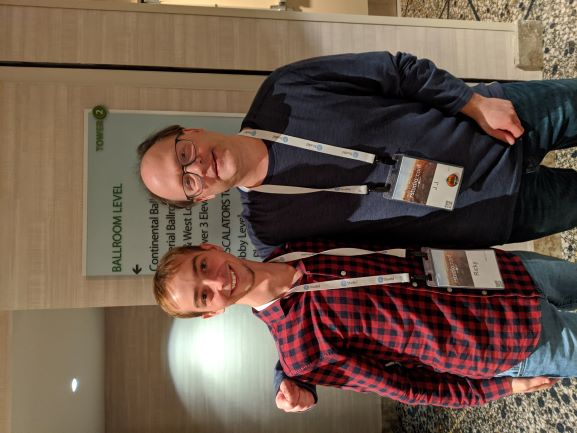
\includegraphics{images/pic_with_jj.jpg}

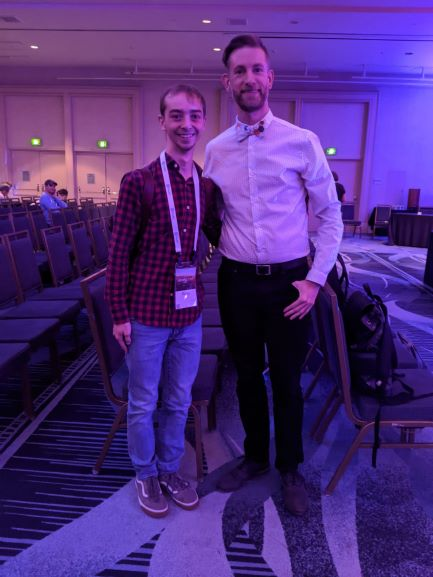
\includegraphics{images/pic_with_hadley.jpg}

Would have loved one with Yihui as well, so I will try and get one with him at next year's conference if I get the chance

\hypertarget{projects-well-suited-for}{%
\chapter{Projects Well Suited For}\label{projects-well-suited-for}}

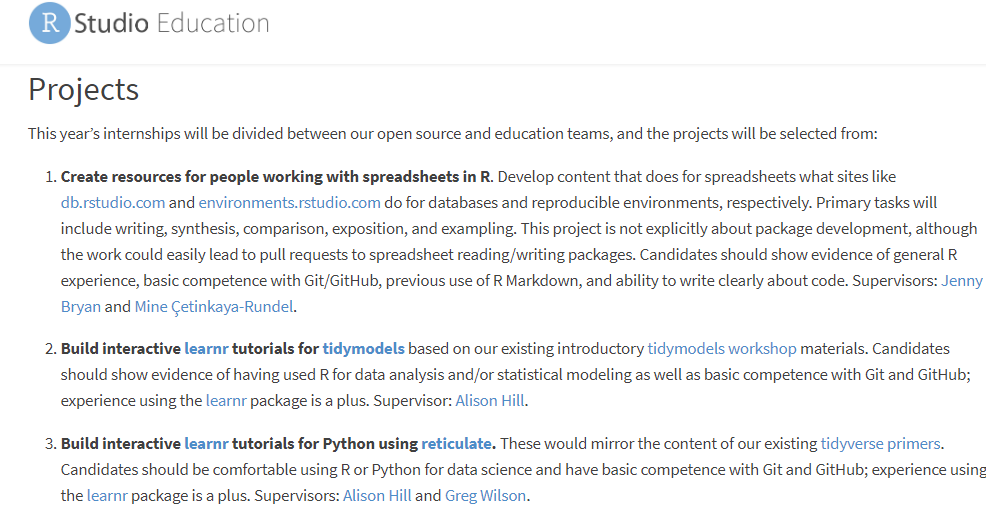
\includegraphics{images/projects_list.png}

\hypertarget{create-resources-for-people-working-with-spreadsheets-in-r}{%
\section{Create resources for people working with spreadsheets in R}\label{create-resources-for-people-working-with-spreadsheets-in-r}}

Here make a guide using github environments making a repo. Maybe a learnr tutorial?

Also put some code here:

\begin{Shaded}
\begin{Highlighting}[]
\KeywordTok{library}\NormalTok{(googlesheets4)}
\NormalTok{practice_sheet <-}\StringTok{ }\KeywordTok{read_sheet}\NormalTok{(}\StringTok{"https://docs.google.com/spreadsheets/d/1_zRBFrB1au7qhxuDDfDuh_bPLGd6RLrwOL5oQ3sBBX4/edit?usp=sharing"}\NormalTok{, }\DataTypeTok{sheet =} \StringTok{'coinmetrics_btc_eth'}\NormalTok{)}
\end{Highlighting}
\end{Shaded}

\begin{Shaded}
\begin{Highlighting}[]
\NormalTok{knitr}\OperatorTok{::}\KeywordTok{kable}\NormalTok{(}\KeywordTok{head}\NormalTok{(practice_sheet,}\DecValTok{30}\NormalTok{))}
\end{Highlighting}
\end{Shaded}

\begin{tabular}{l|l|r|r|r|r|r|r|r|r|r|r|r|r|r|r|r|r|r|r|r|r|r|r|r|r|r|r|r|r|r|r|r|r|r|r|r|r|r|r|r|r}
\hline
date & Symbol & AdrActCnt & BlkCnt & BlkSizeByte & BlkSizeMeanByte & CapMVRVCur & CapMrktCurUSD & CapRealUSD & DiffMean & FeeMeanNtv & FeeMeanUSD & FeeMedNtv & FeeMedUSD & FeeTotNtv & FeeTotUSD & HashRate & IssContNtv & IssContPctAnn & IssContUSD & IssTotNtv & IssTotUSD & NVTAdj & NVTAdj90 & PriceBTC & PriceUSD & ROI1yr & ROI30d & SplyCur & TxCnt & TxTfrCnt & TxTfrValAdjNtv & TxTfrValAdjUSD & TxTfrValMeanNtv & TxTfrValMeanUSD & TxTfrValMedNtv & TxTfrValMedUSD & TxTfrValNtv & TxTfrValUSD & VtyDayRet180d & VtyDayRet30d & VtyDayRet60d\\
\hline
2020-02-24 & BTC & 758122 & 141 & 161000000 & 1141214.00 & 1.657654 & 176000000000 & 106000000000.000000 & 15500000000000.000000 & 0.0000701 & 0.675891 & 0.0000327 & 0.315779 & 22.98117 & 221722.50 & 109000000.000000 & 1762.5 & 3.527725 & 17004614 & 1762.50000 & 17004614.0000 & 84.831600 & 99.54248 & 1.00000 & 9648.00800 & 156.9935 & 15.617360 & 18235605 & 328045.0 & 715274 & 214962.400000 & 2070000000.0000 & 0.771733 & 7445.688000 & 0.009028 & 87.09816 & 552000.700000 & 5330000000.000000 & 0.029542 & 0.026914 & 0.026957\\
\hline
2020-02-24 & ETH & 320273 & 6481 & 153000000 & 23637.33 & 29000000000.000000 & 2310000000000000 & 0.000595 & 0.157336 & 0.0002880 & 0.076260 & 409.2793000 & 108200.000000 & 173.56180 & 13534.88 & 4.497530 & 3578177.0 & 13534.880000 & 3578177 & 63.55275 & 110.3504 & 0.027401 & 264.36720 & 95.27335 & 64.69273 & 110000000.0000 & 687702.000000 & 330920 & 1728314.0 & 457000000 & 6.278402 & 1659.8030 & 0.050000 & 13.218360 & 2077649.000000 & 549000000.00000 & 0.037845 & 0.042600 & 0.039816 & NA & NA\\
\hline
2020-02-23 & BTC & 622397 & 142 & 131000000 & 924118.80 & 1.713841 & 182000000000 & 106000000000.000000 & 15500000000000.000000 & 0.0000586 & 0.584008 & 0.0000260 & 0.259493 & 16.93047 & 168844.90 & 110000000.000000 & 1775.0 & 3.553275 & 17701795 & 1775.00000 & 17701795.0000 & 123.959600 & 102.79560 & 1.00000 & 9972.84200 & 142.6393 & 18.394630 & 18233842 & 289114.0 & 620605 & 147095.100000 & 1470000000.0000 & 0.837293 & 8350.191000 & 0.007532 & 75.11635 & 519628.200000 & 5180000000.000000 & 0.029626 & 0.026096 & 0.026499\\
\hline
2020-02-23 & ETH & 311622 & 6532 & 130000000 & 19886.52 & 30200000000.000000 & 2270000000000000 & 0.000597 & 0.164057 & 0.0003160 & 0.086829 & 361.7215000 & 99466.050000 & 171.31340 & 13640.25 & 4.533300 & 3750791.0 & 13640.250000 & 3750791 & 91.04735 & 116.0288 & 0.027573 & 274.97960 & 74.55645 & 69.48150 & 110000000.0000 & 606290.000000 & 328227 & 1206246.0 & 332000000 & 4.387743 & 1206.5400 & 0.032980 & 9.068855 & 1440176.000000 & 396000000.00000 & 0.038169 & 0.041610 & 0.039251 & NA & NA\\
\hline
2020-02-22 & BTC & 660812 & 148 & 136000000 & 919925.90 & 1.663798 & 176000000000 & 106000000000.000000 & 15500000000000.000000 & 0.0000596 & 0.577093 & 0.0000286 & 0.276422 & 17.90380 & 173223.70 & 114000000.000000 & 1850.0 & 3.703655 & 17899211 & 1850.00000 & 17899211.0000 & 139.355300 & 99.04668 & 1.00000 & 9675.24900 & 145.0484 & 15.644330 & 18232067 & 300166.0 & 664760 & 130831.500000 & 1270000000.0000 & 0.574743 & 5560.784000 & 0.008648 & 83.67068 & 382066.300000 & 3700000000.000000 & 0.029571 & 0.025680 & 0.026337\\
\hline
2020-02-22 & ETH & 314925 & 6528 & 131000000 & 20003.89 & 28700000000.000000 & 2280000000000000 & 0.000505 & 0.132280 & 0.0002100 & 0.055092 & 306.1660000 & 80143.050000 & 172.16340 & 13672.50 & 4.544615 & 3578960.0 & 13672.500000 & 3578960 & 115.77480 & 109.7098 & 0.027055 & 261.76340 & 77.99367 & 61.42636 & 110000000.0000 & 605859.000000 & 315424 & 948495.8 & 248000000 & 3.519405 & 921.2514 & 0.039765 & 10.409090 & 1110105.000000 & 291000000.00000 & 0.038014 & 0.041281 & 0.039218 & NA & NA\\
\hline
2020-02-21 & BTC & 768521 & 154 & 164000000 & 1065423.00 & 1.668813 & 177000000000 & 106000000000.000000 & 15500000000000.000000 & 0.0000697 & 0.675896 & 0.0000330 & 0.320159 & 23.78366 & 230744.20 & 119000000.000000 & 1925.0 & 3.854035 & 18675960 & 1925.00000 & 18675960.0000 & 94.508050 & 99.12436 & 1.00000 & 9701.79800 & 149.2586 & 12.186740 & 18230217 & 341390.0 & 740148 & 192895.900000 & 1870000000.0000 & 0.764840 & 7420.324000 & 0.009278 & 90.01793 & 566094.900000 & 5490000000.000000 & 0.029634 & 0.026571 & 0.026408\\
\hline
2020-02-21 & ETH & 323587 & 6475 & 144000000 & 22264.03 & 29200000000.000000 & 2240000000000000 & 0.000511 & 0.135858 & 0.0002100 & 0.055841 & 342.5926000 & 91098.610000 & 167.68750 & 13564.38 & 4.509210 & 3606895.0 & 13564.380000 & 3606895 & 66.85636 & 111.9210 & 0.027408 & 265.90940 & 85.17202 & 58.70903 & 110000000.0000 & 670542.000000 & 321502 & 1642300.0 & 437000000 & 6.075972 & 1615.6580 & 0.050079 & 13.316370 & 1953437.000000 & 519000000.00000 & 0.037999 & 0.041843 & 0.039089 & NA & NA\\
\hline
2020-02-20 & BTC & 766448 & 126 & 158000000 & 1254015.00 & 1.654352 & 175000000000 & 106000000000.000000 & 15500000000000.000000 & 0.0000874 & 0.840262 & 0.0000407 & 0.391099 & 27.26710 & 262146.70 & 97376948.000000 & 1575.0 & 3.153600 & 15142097 & 1575.00000 & 15142097.0000 & 74.087210 & 98.01293 & 1.00000 & 9614.03000 & 144.5314 & 10.115400 & 18228292 & 311982.0 & 691890 & 246038.300000 & 2370000000.0000 & 0.920950 & 8854.045000 & 0.009867 & 94.86067 & 637196.400000 & 6130000000.000000 & 0.029628 & 0.026662 & 0.026613\\
\hline
2020-02-20 & ETH & 317504 & 6480 & 152000000 & 23416.70 & 28400000000.000000 & 2270000000000000 & 0.000747 & 0.193184 & 0.0003150 & 0.081469 & 515.0929000 & 133219.400000 & 170.24430 & 13579.44 & 4.514685 & 3512075.0 & 13579.440000 & 3512075 & 48.60951 & 109.8569 & 0.026902 & 258.63190 & 75.71038 & 52.88131 & 110000000.0000 & 689600.000000 & 321526 & 2258502.0 & 584000000 & 8.736648 & 2259.5760 & 0.060037 & 15.527460 & 2809060.000000 & 727000000.00000 & 0.038004 & 0.042019 & 0.039459 & NA & NA\\
\hline
2020-02-19 & BTC & 792783 & 141 & 164000000 & 1164743.00 & 1.657941 & 176000000000 & 106000000000.000000 & 15500000000000.000000 & 0.0000921 & 0.887186 & 0.0000431 & 0.415601 & 31.31333 & 301735.40 & 109000000.000000 & 1762.5 & 3.529550 & 16983454 & 1762.50000 & 16983454.0000 & 65.888240 & 98.04085 & 1.00000 & 9636.00200 & 147.3665 & 11.576120 & 18226717 & 340104.0 & 741299 & 276630.800000 & 2670000000.0000 & 1.082174 & 10427.840000 & 0.009287 & 89.48686 & 802214.800000 & 7730000000.000000 & 0.029689 & 0.026677 & 0.027149\\
\hline
2020-02-19 & ETH & 333141 & 6557 & 151000000 & 23009.82 & 28700000000.000000 & 2310000000000000 & 0.000703 & 0.183568 & 0.0002950 & 0.077104 & 489.2541000 & 127733.200000 & 175.63230 & 13800.06 & 4.588780 & 3602884.0 & 13800.060000 & 3602884 & 54.11985 & 111.1964 & 0.027094 & 261.07730 & 82.39645 & 56.40172 & 110000000.0000 & 695837.000000 & 321445 & 2028296.0 & 530000000 & 8.461473 & 2209.0990 & 0.073150 & 19.097810 & 2719898.000000 & 710000000.00000 & 0.038024 & 0.041784 & 0.039517 & NA & NA\\
\hline
2020-02-18 & BTC & 783570 & 150 & 169000000 & 1129523.00 & 1.754254 & 186000000000 & 106000000000.000000 & 15500000000000.000000 & 0.0000939 & 0.957229 & 0.0000306 & 0.311772 & 30.70684 & 313065.50 & 116000000.000000 & 1875.0 & 3.755120 & 19116195 & 1875.00000 & 19116195.0000 & 79.173690 & 104.21180 & 1.00000 & 10195.30000 & 163.7083 & 17.357980 & 18224955 & 327054.0 & 719837 & 230189.500000 & 2350000000.0000 & 0.795163 & 8106.932000 & 0.009234 & 94.14466 & 572388.000000 & 5840000000.000000 & 0.029469 & 0.024237 & 0.025971\\
\hline
2020-02-18 & ETH & 344572 & 6480 & 157000000 & 24219.29 & 31100000000.000000 & 2240000000000000 & 0.000612 & 0.173521 & 0.0002630 & 0.074624 & 449.1443000 & 127361.600000 & 168.17520 & 13619.38 & 4.529285 & 3861978.0 & 13619.380000 & 3861978 & 45.36555 & 121.8865 & 0.027813 & 283.56500 & 96.35371 & 70.01133 & 110000000.0000 & 733983.000000 & 349011 & 2419397.0 & 686000000 & 8.964517 & 2542.0230 & 0.050281 & 14.257880 & 3128715.000000 & 887000000.00000 & 0.037510 & 0.037639 & 0.037625 & NA & NA\\
\hline
2020-02-17 & BTC & 773751 & 157 & 160000000 & 1021988.00 & 1.670618 & 176000000000 & 106000000000.000000 & 15500000000000.000000 & 0.0000736 & 0.712441 & 0.0000306 & 0.296109 & 24.86387 & 240758.80 & 121000000.000000 & 1962.5 & 3.930685 & 19003044 & 1962.50000 & 19003044.0000 & 66.131490 & 99.40991 & 1.00000 & 9683.08000 & 167.2848 & 8.455237 & 18223080 & 337935.0 & 734474 & 275558.300000 & 2670000000.0000 & 1.290830 & 12499.210000 & 0.009700 & 93.92587 & 948080.900000 & 9180000000.000000 & 0.029216 & 0.023312 & 0.025268\\
\hline
2020-02-17 & ETH & 333123 & 6447 & 156000000 & 24137.83 & 29300000000.000000 & 2230000000000000 & 0.000691 & 0.184231 & 0.0003150 & 0.083982 & 480.5111000 & 128108.200000 & 166.68160 & 13581.44 & 4.517240 & 3620923.0 & 13581.440000 & 3620923 & 42.44544 & 116.7915 & 0.027533 & 266.60820 & 100.74940 & 52.28232 & 110000000.0000 & 695366.000000 & 337246 & 2585523.0 & 689000000 & 9.521937 & 2538.6270 & 0.059958 & 15.985200 & 3211235.000000 & 856000000.00000 & 0.037291 & 0.038562 & 0.037104 & NA & NA\\
\hline
2020-02-16 & BTC & 655188 & 142 & 135000000 & 951565.30 & 1.716954 & 181000000000 & 106000000000.000000 & 15500000000000.000000 & 0.0000740 & 0.736494 & 0.0000402 & 0.399774 & 22.16629 & 220600.00 & 110000000.000000 & 1775.0 & 3.555465 & 17664883 & 1775.00000 & 17664883.0000 & 96.007420 & 102.62560 & 1.00000 & 9952.04700 & 177.6229 & 11.663390 & 18221117 & 299527.0 & 635987 & 189788.600000 & 1890000000.0000 & 0.990318 & 9855.687000 & 0.007662 & 76.25218 & 629829.100000 & 6270000000.000000 & 0.029540 & 0.022611 & 0.025111\\
\hline
2020-02-16 & ETH & 337792 & 6552 & 145000000 & 22162.91 & 28700000000.000000 & 2220000000000000 & 0.000897 & 0.234207 & 0.0003150 & 0.082256 & 593.2911000 & 154925.300000 & 168.13720 & 13726.25 & 4.565785 & 3584318.0 & 13726.250000 & 3584318 & 66.14360 & 116.4318 & 0.026239 & 261.12870 & 114.38280 & 52.67612 & 110000000.0000 & 661490.000000 & 317338 & 1658967.0 & 433000000 & 6.623674 & 1729.6310 & 0.061083 & 15.950460 & 2101943.000000 & 549000000.00000 & 0.037491 & 0.038580 & 0.037662 & NA & NA\\
\hline
2020-02-15 & BTC & 736640 & 142 & 154000000 & 1081882.00 & 1.710757 & 181000000000 & 106000000000.000000 & 15500000000000.000000 & 0.0000872 & 0.864220 & 0.0000452 & 0.448010 & 27.63375 & 273898.10 & 110000000.000000 & 1775.0 & 3.555830 & 17593311 & 1775.00000 & 17593311.0000 & 105.823600 & 102.25090 & 1.00000 & 9911.72400 & 178.0282 & 13.683680 & 18219342 & 316931.0 & 690352 & 172167.100000 & 1710000000.0000 & 0.764216 & 7574.694000 & 0.008107 & 80.35445 & 527577.700000 & 5230000000.000000 & 0.029547 & 0.022857 & 0.027785\\
\hline
2020-02-15 & ETH & 343999 & 6472 & 149000000 & 23067.16 & 29100000000.000000 & 2220000000000000 & 0.000713 & 0.188868 & 0.0003300 & 0.087349 & 498.2273000 & 132047.100000 & 166.00290 & 13610.06 & 4.527825 & 3607127.0 & 13610.060000 & 3607127 & 56.04618 & 119.2252 & 0.026739 & 265.03380 & 120.20090 & 61.55386 & 110000000.0000 & 699151.000000 & 341165 & 1957606.0 & 519000000 & 7.010807 & 1858.1010 & 0.051582 & 13.670940 & 2391842.000000 & 634000000.00000 & 0.037546 & 0.038498 & 0.038827 & NA & NA\\
\hline
2020-02-14 & BTC & 741471 & 135 & 149000000 & 1103415.00 & 1.788310 & 189000000000 & 106000000000.000000 & 15500000000000.000000 & 0.0001000 & 1.036332 & 0.0000515 & 0.533520 & 32.91772 & 341080.80 & 104000000.000000 & 1687.5 & 3.380995 & 17485226 & 1687.50000 & 17485226.0000 & 75.228230 & 107.41800 & 1.00000 & 10361.62000 & 190.9000 & 17.592650 & 18217567 & 329123.0 & 719784 & 242164.000000 & 2510000000.0000 & 0.913915 & 9469.636000 & 0.009800 & 101.54380 & 657821.400000 & 6820000000.000000 & 0.029623 & 0.021145 & 0.027669\\
\hline
2020-02-14 & ETH & 323942 & 6493 & 169000000 & 26040.92 & 31200000000.000000 & 2200000000000000 & 0.000678 & 0.193015 & 0.0003150 & 0.089722 & 523.0266000 & 148974.000000 & 165.42620 & 13713.94 & 4.562865 & 3906150.0 & 13713.940000 & 3906150 & 58.01129 & 130.3972 & 0.027489 & 284.83060 & 137.99170 & 71.73600 & 110000000.0000 & 771827.000000 & 342897 & 1891058.0 & 539000000 & 6.868772 & 1956.4370 & 0.060000 & 17.089840 & 2355281.000000 & 671000000.00000 & 0.037251 & 0.035150 & 0.039371 & NA & NA\\
\hline
2020-02-13 & BTC & 815808 & 141 & 171000000 & 1213825.00 & 1.768516 & 186000000000 & 105000000000.000000 & 15500000000000.000000 & 0.0001030 & 1.052676 & 0.0000529 & 0.541663 & 34.63479 & 354504.30 & 109000000.000000 & 1762.5 & 3.531740 & 18040064 & 1762.50000 & 18040064.0000 & 71.231050 & 107.03230 & 1.00000 & 10235.50000 & 186.2207 & 15.915090 & 18215880 & 336765.0 & 732839 & 255729.500000 & 2620000000.0000 & 0.882147 & 9029.211000 & 0.009630 & 98.56784 & 646471.600000 & 6620000000.000000 & 0.029623 & 0.021147 & 0.028125\\
\hline
2020-02-13 & ETH & 374630 & 6481 & 166000000 & 25626.90 & 29400000000.000000 & 2200000000000000 & 0.000709 & 0.189954 & 0.0003420 & 0.091716 & 542.1720000 & 145269.600000 & 164.76990 & 13629.50 & 4.535490 & 3651888.0 & 13629.500000 & 3651888 & 47.96780 & 124.9504 & 0.026178 & 267.94000 & 122.00640 & 61.36300 & 110000000.0000 & 764763.000000 & 373945 & 2286722.0 & 613000000 & 7.504622 & 2010.7880 & 0.060000 & 16.076400 & 2806316.000000 & 752000000.00000 & 0.037149 & 0.034347 & 0.040349 & NA & NA\\
\hline
2020-02-12 & BTC & 822547 & 142 & 165000000 & 1159784.00 & 1.792084 & 189000000000 & 105000000000.000000 & 15500000000000.000000 & 0.0001090 & 1.130271 & 0.0000548 & 0.567839 & 38.29047 & 396694.40 & 110000000.000000 & 1775.0 & 3.556925 & 18389240 & 1775.00000 & 18389240.0000 & 70.962930 & 108.58440 & 1.00000 & 10360.14000 & 188.7519 & 27.557620 & 18214117 & 350973.0 & 775863 & 256670.900000 & 2660000000.0000 & 0.860719 & 8917.162000 & 0.009840 & 101.93980 & 667799.800000 & 6920000000.000000 & 0.029633 & 0.025301 & 0.028023\\
\hline
2020-02-12 & ETH & 394534 & 6463 & 171000000 & 26520.93 & 29200000000.000000 & 2160000000000000 & 0.000742 & 0.197754 & 0.0003170 & 0.084495 & 591.9364000 & 157839.500000 & 161.94990 & 13618.94 & 4.532205 & 3631482.0 & 13618.940000 & 3631482 & 39.45824 & 126.4323 & 0.025738 & 266.64950 & 120.68390 & 85.28875 & 110000000.0000 & 798162.000000 & 401450 & 2779531.0 & 741000000 & 8.800130 & 2346.5500 & 0.075815 & 20.216030 & 3532812.000000 & 942000000.00000 & 0.037149 & 0.041363 & 0.040354 & NA & NA\\
\hline
2020-02-11 & BTC & 885934 & 148 & 185000000 & 1251850.00 & 1.779232 & 187000000000 & 105000000000.000000 & 15500000000000.000000 & 0.0000938 & 0.963561 & 0.0000477 & 0.489677 & 33.94425 & 348682.90 & 114000000.000000 & 1850.0 & 3.707670 & 19003612 & 1850.00000 & 19003612.0000 & 58.744610 & 107.92170 & 1.00000 & 10272.22000 & 186.0850 & 25.814930 & 18212342 & 361869.0 & 784904 & 310025.800000 & 3180000000.0000 & 0.860281 & 8837.002000 & 0.009299 & 95.52171 & 675238.300000 & 6940000000.000000 & 0.029630 & 0.025418 & 0.028299\\
\hline
2020-02-11 & ETH & 319771 & 6534 & 151000000 & 23172.66 & 26100000000.000000 & 2140000000000000 & 0.000600 & 0.142592 & 0.0002520 & 0.059888 & 425.5749000 & 101137.700000 & 162.20530 & 13668.69 & 4.549360 & 3248357.0 & 13668.690000 & 3248357 & 76.62079 & 115.6851 & 0.023135 & 237.64950 & 98.49349 & 63.39239 & 110000000.0000 & 709280.000000 & 348211 & 1431227.0 & 340000000 & 5.190376 & 1233.4910 & 0.050178 & 11.924750 & 1807346.000000 & 430000000.00000 & 0.036184 & 0.037653 & 0.038116 & NA & NA\\
\hline
2020-02-10 & BTC & 703356 & 122 & 146000000 & 1198981.00 & 1.713470 & 180000000000 & 105000000000.000000 & 15500000000000.000000 & 0.0000957 & 0.944549 & 0.0000429 & 0.423623 & 28.26855 & 279077.40 & 93796522.000000 & 1525.0 & 3.056510 & 15055352 & 1525.00000 & 15055352.0000 & 80.946350 & 104.36640 & 1.00000 & 9872.36200 & 171.0681 & 22.912790 & 18210492 & 295461.0 & 639126 & 224969.900000 & 2220000000.0000 & 0.962584 & 9502.973000 & 0.009995 & 98.67199 & 615212.200000 & 6070000000.000000 & 0.029556 & 0.024752 & 0.027949\\
\hline
2020-02-10 & ETH & 318635 & 6592 & 143000000 & 21715.29 & 24600000000.000000 & 2120000000000000 & 0.000586 & 0.131329 & 0.0002640 & 0.059179 & 391.8431000 & 87827.650000 & 161.43200 & 13731.00 & 4.570895 & 3077664.0 & 13731.000000 & 3077664 & 62.92161 & 109.6837 & 0.022704 & 224.13980 & 81.37538 & 56.91004 & 110000000.0000 & 668760.000000 & 305622 & 1742615.0 & 391000000 & 7.245994 & 1624.1160 & 0.066786 & 14.969490 & 2214535.000000 & 496000000.00000 & 0.035934 & 0.036806 & 0.037556 & NA & NA\\
\hline
\end{tabular}

\textbf{This data is sourced from the website \href{https://coinmetrics.io/community-network-data/\#comm-files}{coinmetrics.io}}

They also provide a data dictionary to go along with the data, let's also read that in with \texttt{googlesheets4}:

\begin{Shaded}
\begin{Highlighting}[]
\NormalTok{data_dictionary <-}\StringTok{ }\KeywordTok{read_sheet}\NormalTok{(}\StringTok{"https://docs.google.com/spreadsheets/d/1_zRBFrB1au7qhxuDDfDuh_bPLGd6RLrwOL5oQ3sBBX4/edit?usp=sharing"}\NormalTok{,}\DataTypeTok{sheet =} \StringTok{'coinmetrics_data_dictionary'}\NormalTok{)}
\end{Highlighting}
\end{Shaded}

\begin{Shaded}
\begin{Highlighting}[]
\NormalTok{knitr}\OperatorTok{::}\KeywordTok{kable}\NormalTok{(data_dictionary)}
\end{Highlighting}
\end{Shaded}

\begin{tabular}{l|l|l|l|l|l|l|l|l}
\hline
id & name & category & subcategory & type & unit & interval & interval\_rt & description\\
\hline
AdrActCnt & Addresses, active, count & Addresses & Activity & Sum & Addresses & 1 day & 1 block & The sum count of unique addresses that were active in the network (either as a recipient or originator of a ledger change) that interval. All parties in a ledger change action (recipients and originators) are counted. Individual addresses are not double-counted if previously active.\\
\hline
BlkCnt & Block, count & Blockchain / ledger & Blocks & Sum & Blocks & 1 day & NA & The sum count of blocks created that interval that were included in the main (base) chain.\\
\hline
BlkSizeByte & Block, size, bytes & Blockchain / ledger & Blocks & Sum & Bytes & 1 day & 1 block & The sum of the size (in bytes) of all blocks created that interval.\\
\hline
BlkSizeMeanByte & Block, size, mean, bytes & Blockchain / ledger & Blocks & Mean & Bytes & 1 day & NA & The mean size (in bytes) of all blocks created that day.\\
\hline
CapMVRVCur & Capitalization, MVRV, current supply & Market & Market Capitalization & Ratio & Dimensionless & 1 day & NA & The ratio of the sum USD value of the current supply to the sum "realized" USD value of the current supply.\\
\hline
CapMrktCurUSD & Capitalization, market, current supply, USD & Market & Market Capitalization & Product & USD & 1 day & NA & The sum USD value of the current supply. Also referred to as network value or market capitalization.\\
\hline
CapRealUSD & Capitalization, realized, USD & Market & Market Capitalization & Product & USD & 1 day & NA & The sum USD value based on the USD closing price on the day that a native unit last moved (i.e., last transacted) for all native units.\\
\hline
DiffMean & Difficulty, mean & Mining & Mining & Mean & Dimensionless & 1 day & 1 block & The mean difficulty of finding a hash that meets the protocol-designated requirement (i.e., the difficulty of finding a new block) that interval. The requirement is unique to each applicable cryptocurrency protocol. Difficulty is adjusted periodically by the protocol as a function of how much hashing power is being deployed by miners.\\
\hline
FeeMeanNtv & Fees, transaction, mean, native units & Fees and revenue & Fees & Mean & Native units & 1 day & 1 block & The mean fee per transaction in native units that interval.\\
\hline
FeeMeanUSD & Fees, transaction, mean, USD & Fees and revenue & Fees & Mean & USD & 1 day & 1 block & The USD value of the mean fee per transaction that interval.\\
\hline
FeeMedNtv & Fees, transaction, median, native units & Fees and revenue & Fees & Median & Native units & 1 day & 1 block & The median fee per transaction in native units that interval.\\
\hline
FeeMedUSD & Fees, transaction, median, USD & Fees and revenue & Fees & Median & USD & 1 day & 1 block & The USD value of the median fee per transaction that interval.\\
\hline
FeeTotNtv & Fees, total, native units & Fees and revenue & Fees & Sum & Native units & 1 day & 1 block & The sum of all fees paid to miners that interval. Fees do not include new issuance.\\
\hline
FeeTotUSD & Fees, total, USD & Fees and revenue & Fees & Sum & USD & 1 day & 1 block & The sum USD value of all fees paid to miners that interval. Fees do not include new issuance.\\
\hline
HashRate & Hash rate, mean & Mining & Mining & Mean & Varies & 1 day & NA & The mean rate at which miners are solving hashes that interval. Hash rate is the speed at which computations are being completed across all miners in the network. The unit of measurement varies depending on the protocol.\\
\hline
IssContNtv & Issuance, continuous, native units & Supply & Issuance & Sum & Native units & 1 day & 1 block & The sum of new native units issued that interval. Only those native units that are issued by a protocol-mandated continuous emission schedule are included (i.e., units manually released from escrow or otherwise disbursed are not included).\\
\hline
IssContPctAnn & Issuance, continuous, percent, annualized & Supply & Issuance & Percentage & Dimensionless & 1 year & NA & The percentage of new native units (continuous) issued over that interval, extrapolated to one year (i.e., multiplied by 365), and divided by the current supply at the end of that interval. Also referred to as the annual inflation rate.\\
\hline
IssContUSD & Issuance, continuous, USD & Supply & Issuance & Sum & USD & 1 day & 1 block & The sum USD value of new native units issued that interval. Only those native units that are issued by a protocol-mandated continuous emission schedule are included (i.e., units manually released from escrow or otherwise disbursed are not included).\\
\hline
IssTotNtv & Issuance, total, native units & Supply & Issuance & Sum & Native units & 1 day & 1 block & The sum of all new native units issued that interval.\\
\hline
IssTotUSD & Issuance, total, USD & Supply & Issuance & Sum & USD & 1 day & 1 block & The sum USD value of all new native units issued that interval.\\
\hline
NVTAdj & NVT, adjusted & Valuation & Valuation & Ratio & Dimensionless & 1 day & NA & The ratio of the network value (or market capitalization, current supply) divided by the adjusted transfer value. Also referred to as NVT.\\
\hline
NVTAdj90 & NVT, adjusted, 90d MA & Valuation & Valuation & Ratio & Dimensionless & 1 day & NA & The ratio of the network value (or market capitalization, current supply) to the 90-day moving average of the adjusted transfer value. Also referred to as NVT.\\
\hline
PriceBTC & Price, BTC & Market & Price & NA & BTC & 1 day & 1 block & The fixed closing price of the asset as of 00:00 UTC the following day (i.e., midnight UTC of the current day) for end-of-day data or the closest prior hour (nearest to that block) for block-by-block data, denominated in BTC.\\
\hline
PriceUSD & Price, USD & Market & Price & NA & USD & 1 day & 1 block & The fixed closing price of the asset as of 00:00 UTC the following day (i.e., midnight UTC of the current day) for end-of-day data or the closest prior hour (nearest to that block) for block-by-block data, denominated in USD.\\
\hline
ROI1yr & ROI, percent, 1yr & Market & Returns & Percentage & Dimensionless & 1 year & NA & The return on investment for the asset assuming a purchase 12 months prior\\
\hline
ROI30d & ROI, percent, 30d & Market & Returns & Percentage & Dimensionless & 30 days & NA & The return on investment for the asset assuming a purchase 30 days prior\\
\hline
SplyCur & Supply, current & Supply & Current supply & Sum & Native units & All time & NA & The sum of all native units ever created and visible on the ledger (i.e., issued) as of that interval. For account-based protocols, only accounts with positive balances are counted.\\
\hline
TxCnt & Transactions, count & Transactions & Transactions & Sum & Transactions & 1 day & 1 block & The sum count of transactions that interval. Transactions represent a bundle of intended actions to alter the ledger initiated by a user (human or machine). Transactions are counted whether they execute or not and whether they result in the transfer of native units or not (a transaction can result in no, one, or many transfers). Changes to the ledger mandated by the protocol (and not by a user) or post-launch new issuance issued by a founder or controlling entity are not included here.\\
\hline
TxTfrCnt & Transactions, transfers, count & Transactions & Transfers & Sum & Transfers & 1 day & 1 block & The sum count of transfers that interval. Transfers represent movements of native units from one ledger entity to another distinct ledger entity. Only transfers that are the result of a transaction and that have a positive (non-zero) value are counted.\\
\hline
TxTfrValAdjNtv & Transactions, transfers, value, adjusted, native units & Transactions & Transfer value & Sum & Native units & 1 day & NA & The sum of native units transferred between distinct addresses that interval removing noise and certain artifacts.\\
\hline
TxTfrValAdjUSD & Transactions, transfers, value, adjusted, USD & Transactions & Transfer value & Sum & USD & 1 day & NA & The USD value of the sum of native units transferred between distinct addresses that interval removing noise and certain artifacts.\\
\hline
TxTfrValMeanNtv & Transactions, transfers, value, mean, native units & Transactions & Transfer value & Mean & Native units & 1 day & 1 block & The mean count of native units transferred per transaction (i.e., the mean "size" of a transaction) between distinct addresses that interval.\\
\hline
TxTfrValMeanUSD & Transactions, transfers, value, mean, USD & Transactions & Transfer value & Mean & USD & 1 day & 1 block & The sum USD value of native units transferred divided by the count of transfers (i.e., the mean "size" in USD of a transfer) between distinct addresses that interval.\\
\hline
TxTfrValMedNtv & Transactions, transfers, value, median, native units & Transactions & Transfer value & Median & Native units & 1 day & 1 block & The median count of native units transferred per transfer (i.e., the median "size" of a transfer) between distinct addresses that interval.\\
\hline
TxTfrValMedUSD & Transactions, transfers, value, median, USD & Transactions & Transfer value & Median & USD & 1 day & 1 block & The median USD value transferred per transfer (i.e., the median "size" in USD of a transfer) between distinct addresses that interval.\\
\hline
TxTfrValNtv & Transactions, transfers, value, native units & Transactions & Transfer value & Sum & Native units & 1 day & 1 block & The sum of native units transferred (i.e., the aggregate "size" of all transfers) between distinct addresses that interval.\\
\hline
TxTfrValUSD & Transactions, transfers, value, USD & Transactions & Transfer value & Sum & USD & 1 day & 1 block & The sum USD value of all native units transferred (i.e., the aggregate size in USD of all transfers) between distinct addresses that interval.\\
\hline
VtyDayRet180d & Volatility, daily returns, 180d & Market & Returns & Ratio & Dimensionless & 180 days & NA & The 180D volatility, measured as the standard deviation of the natural log of daily returns over the past 180 days\\
\hline
VtyDayRet30d & Volatility, daily returns, 30d & Market & Returns & Ratio & Dimensionless & 30 days & NA & The 30D volatility, measured as the standard deviation of the natural log of daily returns over the past 30 days\\
\hline
VtyDayRet60d & Volatility, daily returns, 60d & Market & Returns & Ratio & Dimensionless & 60 days & NA & The 60D volatility, measured as the standard deviation of the natural log of daily returns over the past 60 days\\
\hline
\end{tabular}

\textbf{I am comfortable writing packages in R as well as using testthat and showing code coverage for a repository. I attended the building tidy tools workshop working with Charlotte and Hadley at RStudio::conf 2020.}

COULD MAKE THIS FIRST SECTION FROM GOOGLE SHEETS USING DATA ACTUALLY PREDICTING \% CHANGE AND WHATNOT IF I LOAD THAT OTHER DATA INTO HERE. COULD THEN WORK ON NEXT SECTION WHILE MAKING PROGRESS ON BOTH INTERNSHIP AND RESEARCH PAPER!

\hypertarget{build-interactive-learnr-tutorials-for-tidymodels}{%
\section{Build interactive learnr tutorials for tidymodels}\label{build-interactive-learnr-tutorials-for-tidymodels}}

\url{https://education.rstudio.com/blog/2020/02/conf20-intro-ml/}

\url{https://conf20-intro-ml.netlify.com/materials/01-predicting/}

Create parsnip model

\begin{Shaded}
\begin{Highlighting}[]
\KeywordTok{library}\NormalTok{(parsnip)}
\KeywordTok{linear_reg}\NormalTok{() }\OperatorTok\StringTok{              }
\StringTok{  }\KeywordTok{set_engine}\NormalTok{(}\StringTok{"glmnet"}\NormalTok{) }\OperatorTok\StringTok{             }
\StringTok{  }\KeywordTok{set_mode}\NormalTok{(}\StringTok{"regression"}\NormalTok{)}
\end{Highlighting}
\end{Shaded}

\begin{verbatim}
## Linear Regression Model Specification (regression)
## 
## Computational engine: glmnet
\end{verbatim}

\begin{Shaded}
\begin{Highlighting}[]
\CommentTok{# List of models to refer to: https://tidymodels.github.io/parsnip/articles/articles/Models.html}

\NormalTok{xgboost_parsnip <-}\StringTok{ }\KeywordTok{boost_tree}\NormalTok{() }\OperatorTok\StringTok{ }
\StringTok{  }\KeywordTok{set_engine}\NormalTok{(}\StringTok{"xgboost"}\NormalTok{) }\OperatorTok\StringTok{             }
\StringTok{  }\KeywordTok{set_mode}\NormalTok{(}\StringTok{"regression"}\NormalTok{)}
\end{Highlighting}
\end{Shaded}

\hypertarget{build-interactive-learnr-tutorials-for-python-using-reticulate}{%
\section{Build interactive learnr tutorials for Python using reticulate}\label{build-interactive-learnr-tutorials-for-python-using-reticulate}}

Replace this with the Python one:

Could make a very simple xgboost model maybe?

Could also show using Shrimpy API to pull latest data, manipulate in pandas and visualize

Mention experience/courses taken in Python and how it's never clicked with me very much but how I am taking a basic Python course in my Master's in Data Science and I am looking to take it as an opportunity to create a lot of content using reticulate.

\begin{Shaded}
\begin{Highlighting}[]
\KeywordTok{library}\NormalTok{(reticulate)}
\end{Highlighting}
\end{Shaded}

\hypertarget{about-me}{%
\chapter{About Me}\label{about-me}}

\hypertarget{ideal-tutorial}{%
\chapter{Ideal Tutorial}\label{ideal-tutorial}}

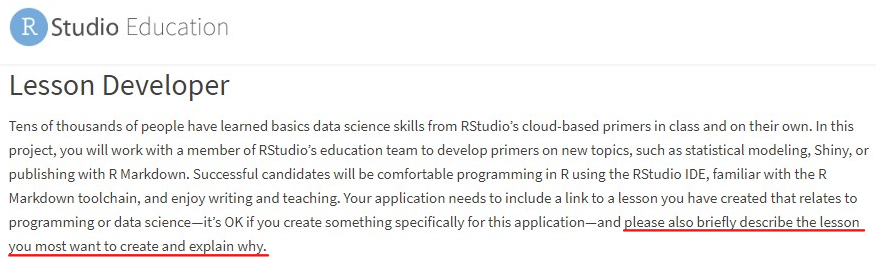
\includegraphics{images/idealTutorial.png}

\hypertarget{cool-charts}{%
\chapter{Cool Charts}\label{cool-charts}}

\hypertarget{disable-while-working-on-bookdown-takes-too-long-to-render}{%
\section{Disable while working on bookdown, takes too long to render!}\label{disable-while-working-on-bookdown-takes-too-long-to-render}}

Here are some examples of charts, which refresh daily using GitHub actions and Netlify for automation.

\begin{verbatim}
## [1] TRUE
\end{verbatim}

  \bibliography{book.bib,packages.bib,main.bib}

\end{document}
